\PassOptionsToPackage{unicode=true}{hyperref} % options for packages loaded elsewhere
\PassOptionsToPackage{hyphens}{url}
%
\documentclass[]{book}
\usepackage{lmodern}
\usepackage{amssymb,amsmath}
\usepackage{ifxetex,ifluatex}
\usepackage{fixltx2e} % provides \textsubscript
\ifnum 0\ifxetex 1\fi\ifluatex 1\fi=0 % if pdftex
  \usepackage[T1]{fontenc}
  \usepackage[utf8]{inputenc}
  \usepackage{textcomp} % provides euro and other symbols
\else % if luatex or xelatex
  \usepackage{unicode-math}
  \defaultfontfeatures{Ligatures=TeX,Scale=MatchLowercase}
\fi
% use upquote if available, for straight quotes in verbatim environments
\IfFileExists{upquote.sty}{\usepackage{upquote}}{}
% use microtype if available
\IfFileExists{microtype.sty}{%
\usepackage[]{microtype}
\UseMicrotypeSet[protrusion]{basicmath} % disable protrusion for tt fonts
}{}
\IfFileExists{parskip.sty}{%
\usepackage{parskip}
}{% else
\setlength{\parindent}{0pt}
\setlength{\parskip}{6pt plus 2pt minus 1pt}
}
\usepackage{hyperref}
\hypersetup{
            pdftitle={Causality and Multiple Regression Supplement},
            pdfauthor={Krista Watts and Kevin Cummiskey},
            pdfborder={0 0 0},
            breaklinks=true}
\urlstyle{same}  % don't use monospace font for urls
\usepackage{longtable,booktabs}
% Fix footnotes in tables (requires footnote package)
\IfFileExists{footnote.sty}{\usepackage{footnote}\makesavenoteenv{longtable}}{}
\usepackage{graphicx,grffile}
\makeatletter
\def\maxwidth{\ifdim\Gin@nat@width>\linewidth\linewidth\else\Gin@nat@width\fi}
\def\maxheight{\ifdim\Gin@nat@height>\textheight\textheight\else\Gin@nat@height\fi}
\makeatother
% Scale images if necessary, so that they will not overflow the page
% margins by default, and it is still possible to overwrite the defaults
% using explicit options in \includegraphics[width, height, ...]{}
\setkeys{Gin}{width=\maxwidth,height=\maxheight,keepaspectratio}
\setlength{\emergencystretch}{3em}  % prevent overfull lines
\providecommand{\tightlist}{%
  \setlength{\itemsep}{0pt}\setlength{\parskip}{0pt}}
\setcounter{secnumdepth}{5}
% Redefines (sub)paragraphs to behave more like sections
\ifx\paragraph\undefined\else
\let\oldparagraph\paragraph
\renewcommand{\paragraph}[1]{\oldparagraph{#1}\mbox{}}
\fi
\ifx\subparagraph\undefined\else
\let\oldsubparagraph\subparagraph
\renewcommand{\subparagraph}[1]{\oldsubparagraph{#1}\mbox{}}
\fi

% set default figure placement to htbp
\makeatletter
\def\fps@figure{htbp}
\makeatother

\usepackage{booktabs}
\usepackage[]{natbib}
\bibliographystyle{apalike}

\title{Causality and Multiple Regression Supplement}
\author{Krista Watts and Kevin Cummiskey}
\date{2021-03-12}

\begin{document}
\maketitle

{
\setcounter{tocdepth}{1}
\tableofcontents
}
\hypertarget{preface}{%
\chapter*{Preface}\label{preface}}
\addcontentsline{toc}{chapter}{Preface}

This textbook supplement is an introduction to causality in statistics and multivariable methods for students in their first college course in statistics. Traditionally, except for a terse warning from instructors that ``correlation does not imply causation'', students only encounter causality in statistics if they take graduate-level courses in certain disciplines (economics, epidemiology, etc.). However, given the ubiquity of data-driven arguments in modern society, a deeper understanding of drawing cause-and-effect conclusions from data is a core competency of college graduates and deserves attention in the liberal arts curriculum. For more on causality in the undergraduate curriculum, see our paper \citep{cummiskey2020causal} and others on this subject \citep{horton2015challenges, kaplan2018teaching, lubke2020we}.

After introducing concepts in causality, we use an example-based approach to multiple regression emphasizing how the scientific goal of the study impacts modeling decisions and interpretation of results. Prediction and cause-and-effect are the two main scientific goals of studies using multiple regression. These goals determine how researchers use and interpret models. However, this distinction is rarely made in introductory courses. Too often, multiple regression in the introductory course focuses on prediction and much of the ``thinking'' outsourced to algorithmic searches. This narrow focus on prediction deprives students of the opportunity to exercise critical judgment and creativity. On the other hand, cause-and-effect studies require tying subject matter knowledge to developing causal models. During this process, students have to carefully consider relationships between variables (which is not particularly important in prediction), thus developing multivariable thinking, an important goal of the revised GAISE report \citep{carver2016guidelines}. Our approach to multiple regression uses the scientific goal to motivate how we think about our data and models. \citet{hernan2019second} argue for this approach in data science education; we believe it is appropriate for introductory statistics courses also.

\hypertarget{introduction}{%
\chapter{Introduction}\label{introduction}}

\hypertarget{goals-of-quantitative-research-describe-predict-cause-and-effect}{%
\section{Goals of quantitative research (describe, predict, cause-and-effect)}\label{goals-of-quantitative-research-describe-predict-cause-and-effect}}

Researchers and practitioners in nearly every discipline employ quantitative methods to answer important questions and make decisions. Regardless if it is finance, medicine, psychology, etc., all researchers typically have one of three goals \citep{cozby2020methods} when they conduct quantitative research:

\begin{itemize}
\item
  \textbf{describe}
\item
  \textbf{predict}
\item
  \textbf{cause-and-effect}
\end{itemize}

For example, consider medical researchers investigating a newly discovered variant of the coronavirus. Initially, they focus on describe studies. \emph{How prevalent is the variant in the population? How does the prevalence vary over space and time? What groups of individuals are most vulnerable to the variant? What else is associated with the variant?} Together, these studies help the researchers better understand the variant and identify important variables for refined predict studies.

Predict studies identify individuals most at risk for the variant or for transmitting it to others. Researchers select potential predictors as inputs to algorithms and statistical methods that transform them into estimates of each individual's risk for the variant. These methods rely upon associations between the inputs and the variant. In addition, these methods estimate the error associated with their predictions. Researchers try to ensure error estimates obtained within their study are good estimates of the error when their models are applied to other populations. While predict studies help us identify who is at risk, they do not tell us the effect if we change something about them (quit smoking, lose weight, etc.) To answer these ``what if?'' questions, researchers use cause-and-effect studies.

Cause-and-effect studies try to estimate the effect of intervening or changing some aspect of an individual. These studies are tremendously important in public policy (where they are aptly called \emph{intervention studies}) to justify legislation and regulations to reduce risk. Unlike prediction studies, which are highly algorithmic and only require researchers to identify appropriate inputs, cause-and-effect studies use subject matter knowledge of the causal structure of the inputs to select appropriate statistical models \citep{hernan2019second}. For example, to assess the affect of quitting smoking on coronavirus risk, we would have to understand why some people quit smoking and others do not, as these reasons themselves may be responsible for some of the reduction in risk we observe between the two groups. Also, unlike prediction studies which rely upon what we \emph{see}, cause-and-effect studies require us to ask what would happen if we \emph{do} something \citep{pearl2018book}. Only human beings are capable of such counterfactual thinking (``what would have happened if'') - even our most sophisticated computer algorithms require human supervision to address cause-and-effect questions.

\textbf{Exercises}

\begin{enumerate}
\def\labelenumi{\arabic{enumi}.}
\tightlist
\item
  For the following studies, identify the goal (describe, predict, cause-and-effect) of the study. Briefly explain your choice:
\end{enumerate}

\begin{itemize}
\item
  \emph{A researcher obtains school records to collect information on the extracurricular activities of students.}
\item
  \emph{A researcher obtains school records to determine the impact of extracurricular activities on grades.}
\item
  \emph{A researcher obtains school records on extracurricular activities to identify students who are at risk to graduate.}
\end{itemize}

\begin{enumerate}
\def\labelenumi{\arabic{enumi}.}
\setcounter{enumi}{1}
\tightlist
\item
  Select an area of interest to you. Write a sentence describing a study in your area of interest for each of the three goals (describe, predict, cause-and-effect)
\end{enumerate}

\hypertarget{validity}{%
\section{Validity}\label{validity}}

\begin{itemize}
\item
  internal validity
\item
  external validity
\end{itemize}

In an area of research, there is often a natural tradeoff between internal and external validity. Our knowledge comes from both observational studies and experiments (trials) -- rarely does a single study answer every question and the two types of studies used together increase our overall knowledge. Consider researchers investigating the effectiveness of Covid-19 vaccines. Initial vaccine trials focus on internal validity to understand its effectiveness against the virus and obtain approval for mass distribution. For example, \citet{polack2020safety} randomly assigned 43,548 persons 16 years of age or older to receive two doses of either placebo or the BNT162b2 vaccine (Pfizer). They observed eight cases of Covid-19 among participants who received BNT162b2 and 162 cases among those who received the placebo. This was a huge moment in the pandemic! However, the subjects in the study were relatively healthy and had volunteered for the trials. From this study alone, the external validity of these results is not clear and researchers want to know if the vaccine results would hold in the general public. Given the success of the trials, it would be unethical to withhold the vaccine from large segments of the population, so observational studies are required.

\citet{dagan2021bnt162b2} conducted an observational study after the mass vaccination campaign in Israel using the health records of 4.7 million patients enrolled in its largest integrated health care organization. The researchers matched vaccine recipients to controls on important variables: age, sex, sector, neighborhood of residence, etc.. In this larger sample, they found vaccine effectiveness results consistent with the randomized trial, thus providing evidence of the vaccine's effectiveness in the general public. The authors specifically address the importance of observational studies:

\begin{quote}
``Although randomized clinical trials {[}experiments{]} are considered the ``gold standard'' for evaluating intervention effects, they have notable limitations of sample size and subgroup analysis, restrictive inclusion criteria, and a highly controlled setting that may not be replicated in a mass vaccine rollout."
\end{quote}

\textbf{Exercises}

\begin{enumerate}
\def\labelenumi{\arabic{enumi}.}
\tightlist
\item
  Read the article \href{https://www.nature.com/articles/d41586-020-02821-4}{``Dozens to be deliberately infected with coronavirus in UK `human challenge' trials''} in Nature News. Write a paragraph discussing issues of internal and external validity.
\end{enumerate}

\hypertarget{causality}{%
\chapter{Causality}\label{causality}}

The last few decades have seen a revolution in how statisticians view causality. A hundred years ago, when the statistical methods students learn in introductory courses were developed, causality was considered outside the realm of statistics, except for the case of randomized controlled experiments. In other words, statistics could only answer questions of association, but not of causality. However, this limited view of statistics was at odds with its usage in every day research. For example, the greatest public health triumph of the 20th century was the reduction in cigarette smoking, which exploded after World War II with their mass production and marketing. The statistical evidence of the health effects of smoking comes entirely from observational studies -- there has never been a randomized controlled trial for smoking. The American Cancer Society's observational studies of the 1960's and 1970's were huge undertakings and provided compelling evidence of the harmful effects of cigarette smoking. Clearly, statistical theory and practice had diverged in their understandings of causality.

However, in the 1980's and 1990's, researchers in different disciplines began revisiting causality. They developed mathematical language for expressing causation, which cannot be uniquely expressed using the traditional language of association. In addition, they showed that randomized controlled trials are special cases of more general situations when the researcher has full knowledge of the assignment mechanism. The \emph{assignment mechanism} is the process in which subjects are assigned to different levels of the treatment. Lastly, they showed that causal effects could be estimated from observational studies under a wide variety of circumstances when the assignment mechanism is known. Today, while ``correlation does not imply causation'' is still useful advice when assessing causal claims in observational studies, statistical theory and practice suggest our assessment of causal claims in observational studies should be much richer and nuanced than this simple rule of thumb.

(add citations)

\hypertarget{what-does-it-mean-for-one-thing-to-cause-another}{%
\section{What does it mean for one thing to cause another}\label{what-does-it-mean-for-one-thing-to-cause-another}}

We say one variable (the treatment or intervention) \emph{causes} another variable (the outcome) if there is a change in the average outcome between subjects when they receive the treatment and the same subjects when they do not receive the treatment. This definition differs from \emph{association}, which is a change in the average outcome between subjects who received the treatment and different subjects who did not receive the treatment. Thus, causation is a comparison of observed outcomes and their counterfactuals (``what would have happened if the subject were in the other treatment group'').

Unfortunately, in most cases, we cannot observe both outcomes for subjects. For example, when estimating the effect of smoking on long term health outcomes, it is impossible to observe the same subject as a smoker and as a nonsmoker. We only observe one of the outcomes. However, under certain circumstances, we can obtain good estimates of effects without observing both outcomes for each individual. The most famous of these is the randomized controlled experiment.

(add see and do from Pearl here?)

\hypertarget{randomized-controlled-experiments}{%
\section{Randomized controlled experiments}\label{randomized-controlled-experiments}}

One of the most important scientific discoveries of the early 20th century was the randomized controlled trial (RCT). In its simplest form, researchers randomly assign subjects to receive the treatment or be in the control group. If they observe a difference in average outcomes between the two groups, then we would say the treatment caused the outcome. \emph{Why does assigning subjects to groups by the simple action of flipping a coin result in such a radical difference in how we interpret the results?} The answer lies in the definition of causation above. Causation compares the outcomes between the same subjects. When we randomize the treatment, we end up comparing the outcomes between one group of subjects with the treatment and another group of subjects without the treatment who we expect to be very similar. In fact, when we have large enough sample sizes, it would be very unusual for the two groups to differ much. We refer to the two groups as \emph{exchangeble}. In other words, we would expect the control group to have had similar results as the treatment group if they were the treatment group, and vice versa.

However, an overly restrictive view of causality followed this important discovery. That is, causality can \emph{only} be shown with RCTs. This placed a huge limitation on the types of research questions statistics could address. Frequently, RCTs are not ethical, feasible, or desirable. Imagine enrolling in a study where you could be randomly assigned to be a smoker for the next 20 years. Towards the end of the 20th century, researchers began taking a more expansive view of causality in observational studies.

\hypertarget{observational-studies-and-confounding}{%
\section{Observational Studies and Confounding}\label{observational-studies-and-confounding}}

In observational studies, researchers do not intervene on the assignment of subjects to treatment and control groups. (Note: a common misconception is that observational studies do not have treatment and control groups. This is not true. It is about how subjects are \emph{assigned} to the treatment groups.) Instead, other factors determine subjects' group (treatment or control) assignment. Confounding occurs when these other factors determining assignment are themselves causes of the outcome. In other words, the treatment and control groups are different in ways that are important to the outcome. The two groups are not exchangeable. An observed association between the treatment and outcome could mean (1) the treatment caused the outcome, (2) other factors causing group assignment caused the outcome, or (3) both. Furthermore, with only information on the treatment and outcome, it is not possible to identify which of the three is the correct explanation. Confounding is a form of statistical bias -- using the observed association as an estimate of the treatment effect will be systemically off. Increasing the sample size does not help fix bias, you just get a more precise, wrong estimate.

For example, consider an observational study investigating long term health effects of smoking. In many populations, males are more likely to be smokers. In addition, males have different risks for long term health outcomes than females, regardless of whether they smoke. If we observe an association between smoking and an outcome without information on sex, we cannot distinguish the effect of smoking from the effect of sex.

However, researchers in the late 20th century had a key insight. If we know the assignment mechanism and measure a sufficient set of confounding variables, you can obtain good estimates of treatment effects from observational studies. This was huge! Observational studies and RCTs are not fundamentally different. Estimating effects requires understanding the assignment mechanism, and RCTs are just a special case with a simple, known assignment mechanism. Given this insight, researchers became more comfortable making causal claims from observational studies when they have knowledge of the assignment mechanism. \emph{How do we identify a sufficient set of confounding variables?} For that question, we turn to causal diagrams.

(discuss well-defined interventions?)

\hypertarget{causal-diagrams}{%
\section{Causal Diagrams}\label{causal-diagrams}}

Causal diagrams are useful tools for depicting the assignment mechanism (also called the causal model). Experts use subject matter knowledge in their field to specify the causal model. They typically specify the causal model prior to collecting data to identify confounding variables to measure. Importantly, there is no way to determine the presence of unmeasured confounding using the data. In addition, using simple heuristics for causal diagrams, they identify a sufficient set of confounding variables to control for during design and analysis.

Causal diagrams are directed, acyclic graphs (DAGs) where the nodes are variables and a directed edge (arrow) connecting two nodes indicates the node at the arrow's tail is a cause of the node at the arrow's head. The graphs are directed because the arrows point in one direction. They are acyclic because you can never get back to where you started by following arrows. The convention in many disciplines is to order the variables temporally from left to right -- we adopt that convention here.

There are three building blocks of causal diagrams.

\hypertarget{confounding-variable}{%
\subsection{Confounding variable}\label{confounding-variable}}

Figure \ref{fig:confounder} depicts the confounding variable \(C\) of the effect of treatment \(X\) on outcome \(Y\). We will observe an association between \(X\) and \(Y\) even if there is no treatment effect. The levels of \(X\) differ in terms of \(C\) and \(C\) itself is a cause of \(Y\). Without measuring and controlling for \(C\), we cannot distinguish the effect of \(X\) on \(Y\) from the association through confounding variable \(C\). However, if \(C\) is the only confounding variable, controlling for it will result in good estimates of the effect of \(X\) on \(Y\).

(backdoor path)

\begin{figure}
\centering
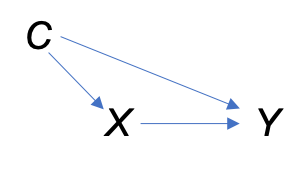
\includegraphics{./images/confounder.png}
\caption{\label{fig:confounder} A confounding variable \(C\) on the effect of \(X\) on \(Y\).}
\end{figure}

For example, let's say researchers investigate the effect of a master's degree on adult earnings. They survey a large number of individuals and record whether they have a master's degree and their earnings. Socioeconomic status is a confounding variable. Individuals with higher socioeconomic status are more likely to earn master's degrees. In addition, they are more likely to have higher adult earnings, regardless of whether they have a master's degree. For this example, let's assume socioeconomic status is the only confounding variable. If the researchers observe an association between master's degrees and earnings without information on socioeconomic status, it is not possible to determine if the association is due to an effect of master's degrees or the effect of socioeconomic status.

\hypertarget{collider}{%
\subsection{Collider}\label{collider}}

Figure \ref{fig:collider} depicts treatment \(X\) with no effect on outcome \(Y\). \(X\) and \(Y\) are both causes of collider \(Z\) (the two incoming arrows \emph{collide}). The box around \(Z\) indicates conditioning upon \(Z\) in the analysis. In this case, there will be an association between \(X\) and \(Y\) even though there is no treatment effect. Figure \ref{fig:collider} is a common way to depict \emph{selection bias} where an association in subjects selected for the study is not present in the general population. In the selection bias diagram, \(Z\) is an indicator of selection into the study with a box around it because researchers only observe subjects selected into the study.

\begin{figure}
\centering
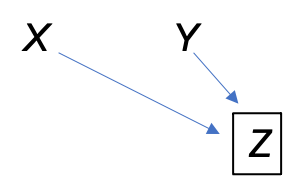
\includegraphics{./images/collider.png}
\caption{\label{fig:collider} Collider \(Z\) with no treatment effect of \(X\) on \(Y\).}
\end{figure}

A very famous example appears in \citet{pearl2018book}. In the general population, we would not expect to see an association between an individual's talent and looks. More talented people are not better looking and vice versa. However, if we look only at famous Hollywood actors (\(Z\)), we would see an association between talent and looks in this group because an individual needs either talent or looks (or both) to become a famous Hollywood actor. More seriously, \emph{selection bias} is a huge issue in medical and public health studies resulting in easily misinterpretated associations \citep{hernan2004structural, cole2010illustrating, elwert2014endogenous}.

\hypertarget{mediator}{%
\subsection{Mediator}\label{mediator}}

Figure \ref{fig:mediator} depicts mediator \(M\) of the effect of treatment \(X\) on outcome \(Y\). In this case, \(X\) is a cause of \(M\), \(M\) is a cause of \(Y\), and there is no effect of \(X\) on \(Y\) that cannot be explained by the effect of \(M\) on \(Y\). A common mistake is to adjust for \(M\). If \(M\) is categorical, we will not observe an association between \(X\) and \(Y\) within levels of \(M\). However, there is still an effect of \(X\) on \(Y\).

\begin{figure}
\centering
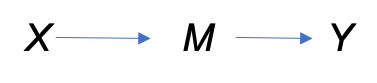
\includegraphics{./images/mediator.png}
\caption{\label{fig:mediator} Mediator \(M\) of the effect of treament \(X\) on outcome \(Y\).}
\end{figure}

For example, let's say researchers are investigating an adverse reaction to a medication using a treatment group and a control group where the adverse reactions are always preceeded by increased blood pressure. Even if there is an effect of the medication on the adverse reason, when we condition upon experiencing increased blood pressure, we will not observe an association between the medication and adverse reactions.

Unfortunately, some researchers condition upon everything that they measure, often resulting in poor estimates of effects \citep{hernan2002causal}.

\hypertarget{matching}{%
\chapter{Matching}\label{matching}}

Chapter on matching

\hypertarget{categorical}{%
\chapter{(COL Watts) Quantitative explanatory variable with categorical confounding variable}\label{categorical}}

Introduce multiple regression by adding a categorical confounding variable

Explanatory (\(X\)) - quantitative

Response (\(Y\)) - quantitative

Confounding (\(C\)) - categorical

\hypertarget{unadjusted-effect-of-x-on-y}{%
\section{\texorpdfstring{Unadjusted effect of \(X\) on \(Y\)}{Unadjusted effect of X on Y}}\label{unadjusted-effect-of-x-on-y}}

short review of simple regression

\hypertarget{effect-of-x-and-y-adjusting-for-c.}{%
\section{\texorpdfstring{Effect of \(X\) and \(Y\) adjusting for \(C\).}{Effect of X and Y adjusting for C.}}\label{effect-of-x-and-y-adjusting-for-c.}}

\hypertarget{assessing-model-adequacy}{%
\section{Assessing model adequacy}\label{assessing-model-adequacy}}

\hypertarget{interactions}{%
\chapter{(Kevin) Interactions}\label{interactions}}

Extend the example in the last chapter\ldots{}introduce in terms of effect modification. We have a new research question, ``does the affect of \(X\) on \(Y\) change based on another variable of interest?''

\hypertarget{activity}{%
\chapter{Activity}\label{activity}}

\emph{Title}: The Indoor Obstacle Course Test (IOCT)

\emph{Topics}\}*: Confounding, Causal Diagrams, Simple Linear Regression, Confidence Intervals

\emph{Background}: Cadets at West Point must pass the \href{https://www.youtube.com/watch?v=94tPO0fGtJo\&t=77s}{Indoor Obstacle Course Test} (IOCT) to graduate. The IOCT begins with a series of floor and climbing obstacles and ends with several laps around an indoor track. It is an exhausting test of endurance and strength. In addition to being a graduation requirement, cadets receive a letter grade that is factored into their class rank.

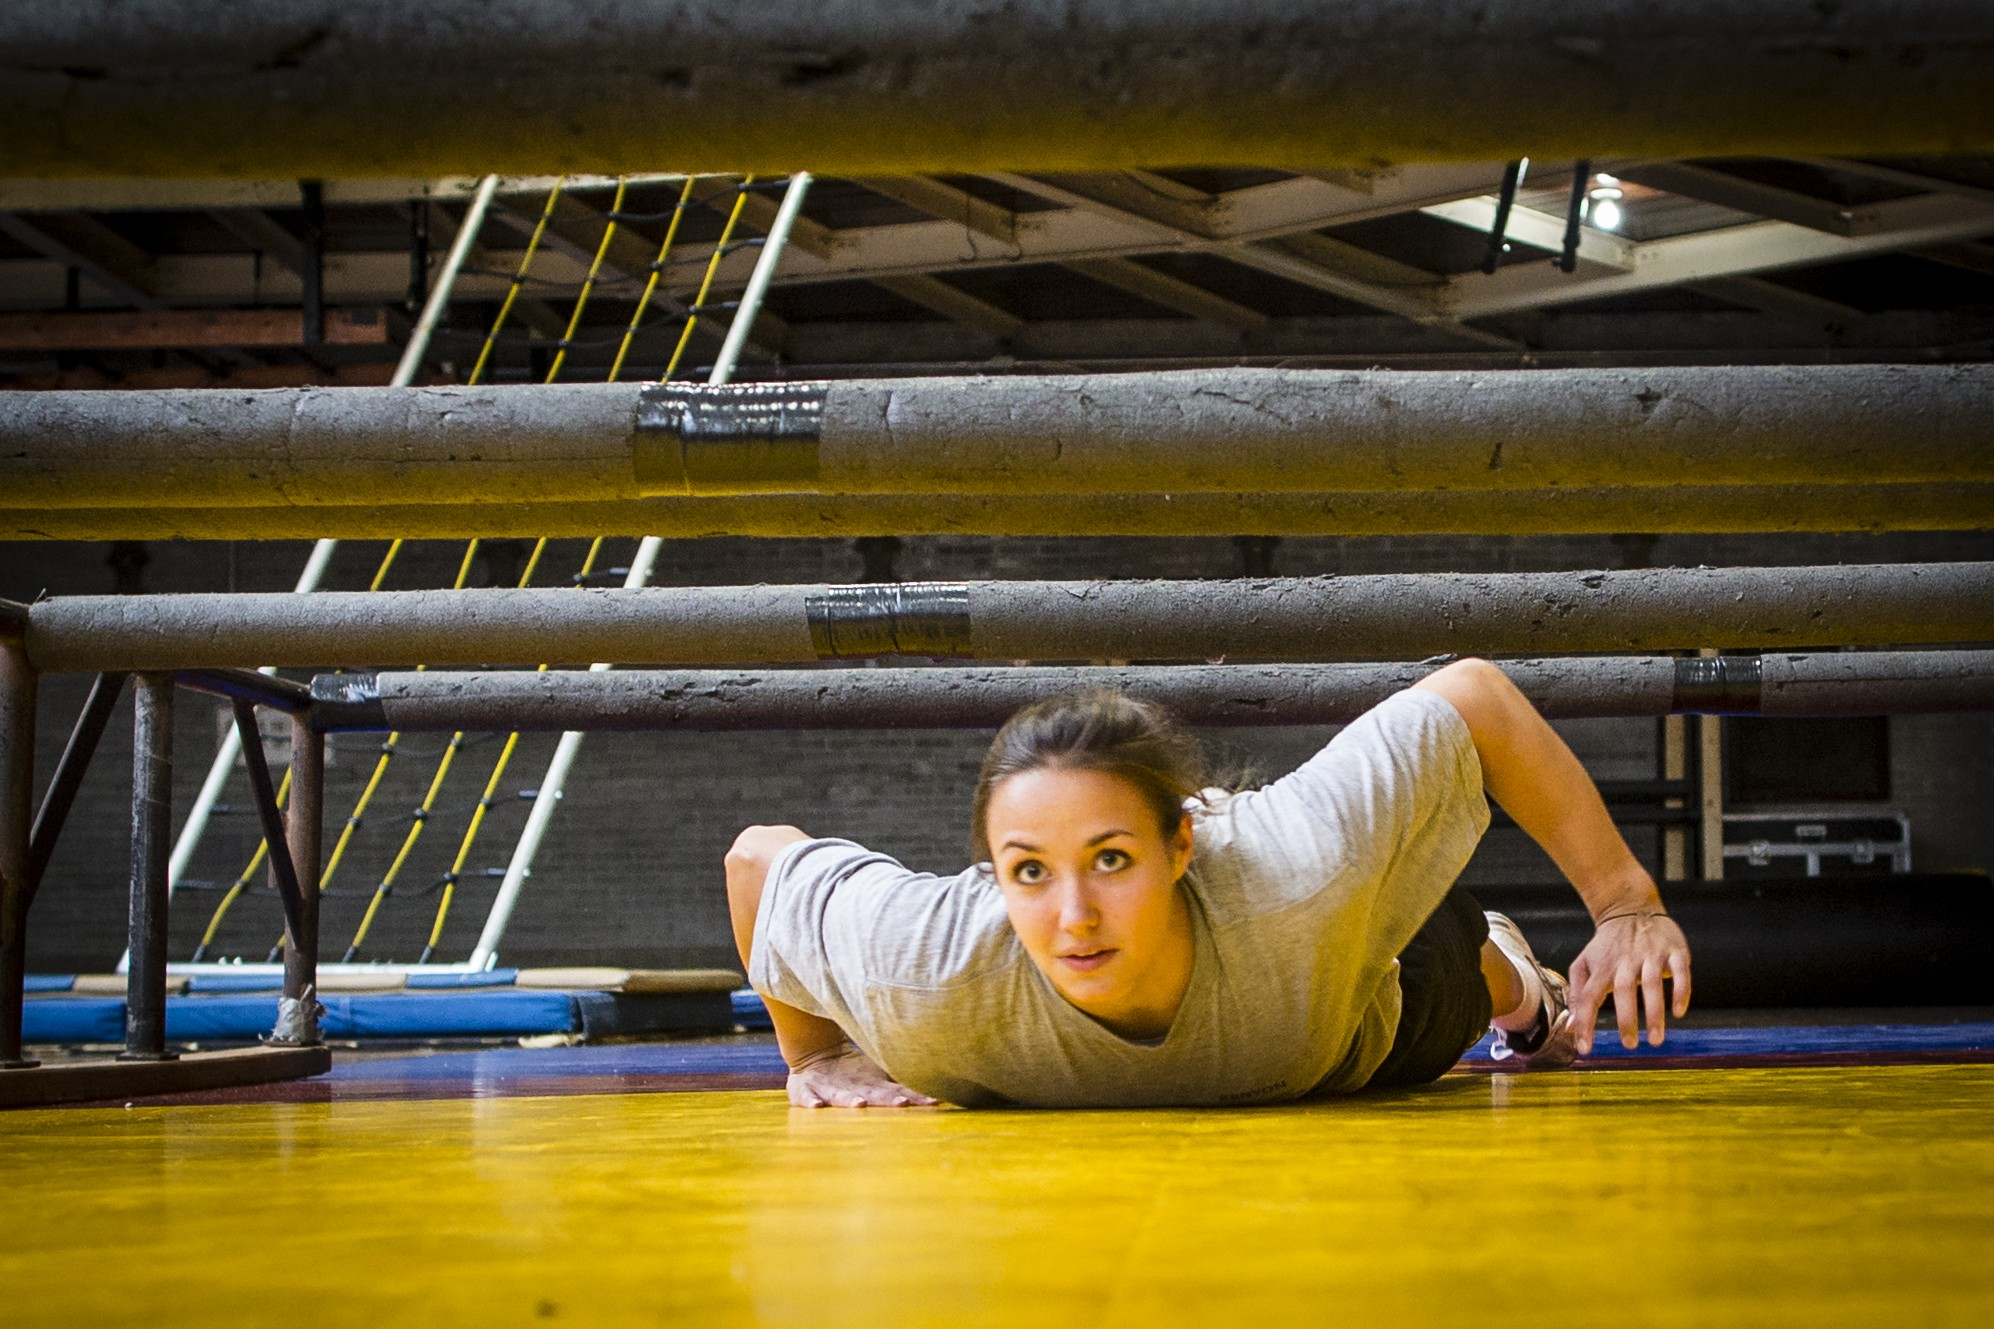
\includegraphics[width=0.5\textwidth,height=\textheight]{./images/crawlObstacle.jpg} 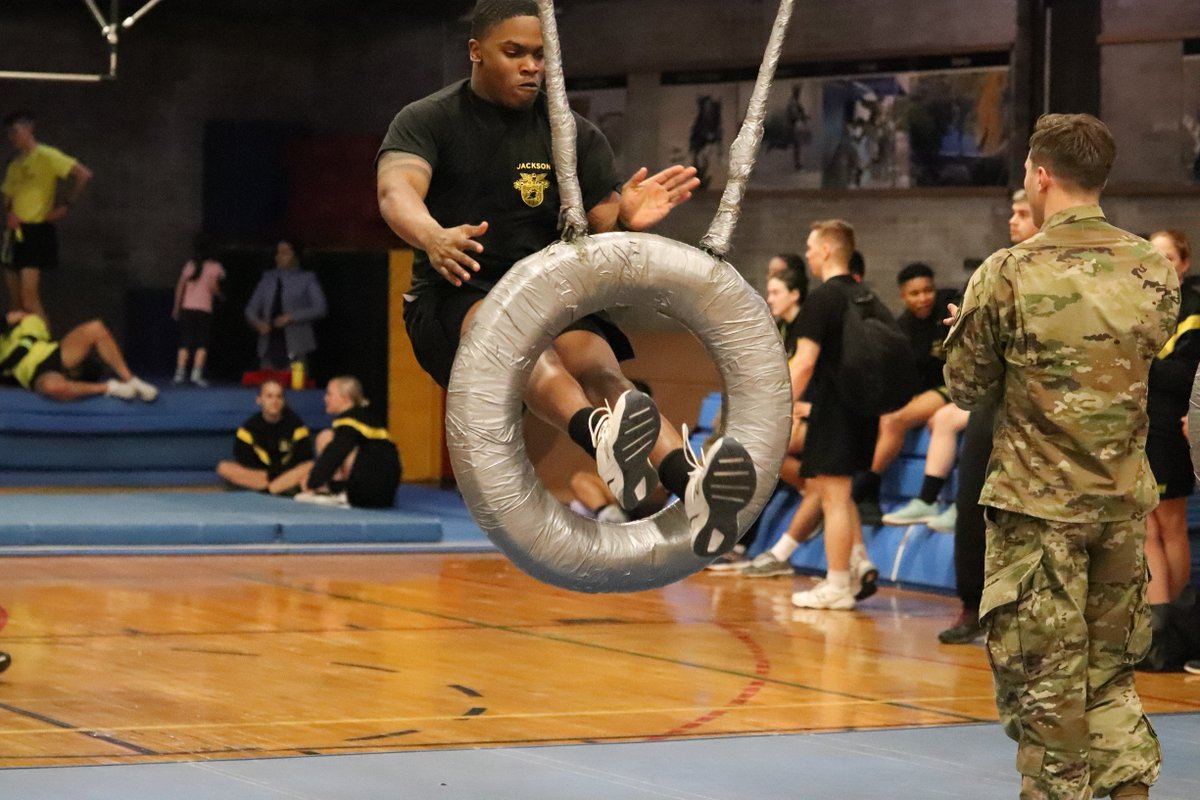
\includegraphics[width=0.5\textwidth,height=\textheight]{./images/tireObstacle.jpg}

Shorter cadets often argue they are at a disadvantage on the obstacle course. Many obstacles appear to favor taller cadets because they are easier to reach. In this study, we will investigate the effect of height on IOCT times.

\begin{enumerate}
\def\labelenumi{\arabic{enumi}.}
\tightlist
\item
  \href{https://www.youtube.com/watch?v=94tPO0fGtJo\&t=77s}{Watch the video of Cadet Madaline Kenyon running the IOCT}. In your opinion, do some obstacles favor taller cadets? Explain.
\end{enumerate}

\vspace{1in}

The file \texttt{obstacle\_course.csv} contains height (inches), IOCT times (seconds), biological sex (M/F), and whether the cadet played an intercollegiate sport for a sample of 384 cadets who ran the IOCT course in the last five years.

\begin{enumerate}
\def\labelenumi{\arabic{enumi}.}
\setcounter{enumi}{1}
\tightlist
\item
  What is the explanatory variable in this study? Classify the variable as quantitative or categorical.
\end{enumerate}

\vspace{0.25in}

\begin{enumerate}
\def\labelenumi{\arabic{enumi}.}
\setcounter{enumi}{2}
\tightlist
\item
  What is the response variable in this study? Classify the variable as quantitative or categorical.
\end{enumerate}

\vspace{0.25in}

\begin{enumerate}
\def\labelenumi{\arabic{enumi}.}
\setcounter{enumi}{3}
\tightlist
\item
  Is this study an observational study or a randomized experiment? Explain.
\end{enumerate}

\vspace{1in}

\newpage

Figure 1 depicts IOCT times in seconds versus height in inches. Table 1 contains information from the linear regression model.

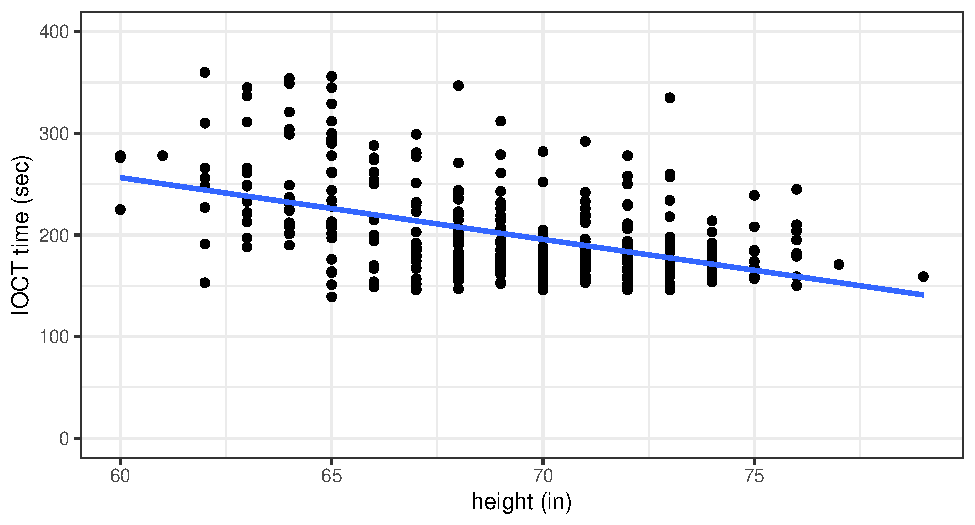
\includegraphics{MA206supplement_files/figure-latex/unnamed-chunk-2-1.pdf}

\begin{table}

\caption{\label{tab:unnamed-chunk-2}Linear regression output for IOCT times and height.}
\centering
\begin{tabular}[t]{l|r|r|r|r}
\hline
term & estimate & std.error & statistic & p.value\\
\hline
(Intercept) & 621.00 & 39.98 & 15.53 & 0\\
\hline
height & -6.08 & 0.58 & -10.52 & 0\\
\hline
\end{tabular}
\end{table}

\begin{enumerate}
\def\labelenumi{\arabic{enumi}.}
\setcounter{enumi}{4}
\item
  Interpret the estimate of the height coefficient in Table 1.

  \vspace{1in}
\item
  Calculate and interpret a 95\% confidence interval for the slope coefficient.
\end{enumerate}

\vspace{1in}

\newpage

\begin{enumerate}
\def\labelenumi{\arabic{enumi}.}
\setcounter{enumi}{6}
\tightlist
\item
  The \(p\)-value for height in Table 1 indicates there is strong evidence of an association between height and IOCT time. Taller cadets tend to do better on the IOCT. Some people would say the result is \emph{statistically significant}. However, statistical significance and practical signifigance are different. \href{https://en.wikipedia.org/wiki/Indoor_Obstacle_Course_Test}{Review the grade scale for the IOCT.} In your opinion, does the observed association have practical significance? Explain.
\end{enumerate}

\vspace{1in}

\begin{enumerate}
\def\labelenumi{\arabic{enumi}.}
\setcounter{enumi}{7}
\tightlist
\item
  A shorter cadet argues Figure 1 shows evidence the IOCT is unfair based on height. Do you agree or disagree? Explain.
\end{enumerate}

\vspace{1in}

\begin{enumerate}
\def\labelenumi{\arabic{enumi}.}
\setcounter{enumi}{8}
\tightlist
\item
  Briefly explain the difference between these two conclusions.
\end{enumerate}

\begin{itemize}
\item
  \emph{Height is associated with faster IOCT times.}
\item
  \emph{Height causes faster IOCT times.}
\end{itemize}

\vspace{1in}

\begin{enumerate}
\def\labelenumi{\arabic{enumi}.}
\setcounter{enumi}{9}
\tightlist
\item
  Based on the analysis presented thus far, is it possible to distinguish between these two explanations? Explain.
\end{enumerate}

\vspace{1in}

\begin{enumerate}
\def\labelenumi{\arabic{enumi}.}
\setcounter{enumi}{10}
\tightlist
\item
  Draw a causal diagram depicting the relationship between height, IOCT time, and sex. Explain your decisions to include/exclude arrows in the diagram.
\end{enumerate}

\vspace{1in}

\begin{enumerate}
\def\labelenumi{\arabic{enumi}.}
\setcounter{enumi}{11}
\tightlist
\item
  Based on your diagram, identify the confounding variable.
\end{enumerate}

\vspace{0.5in}

Below are boxplots of height in inches and IOCT times in seconds by sex.

\begin{figure}
\centering
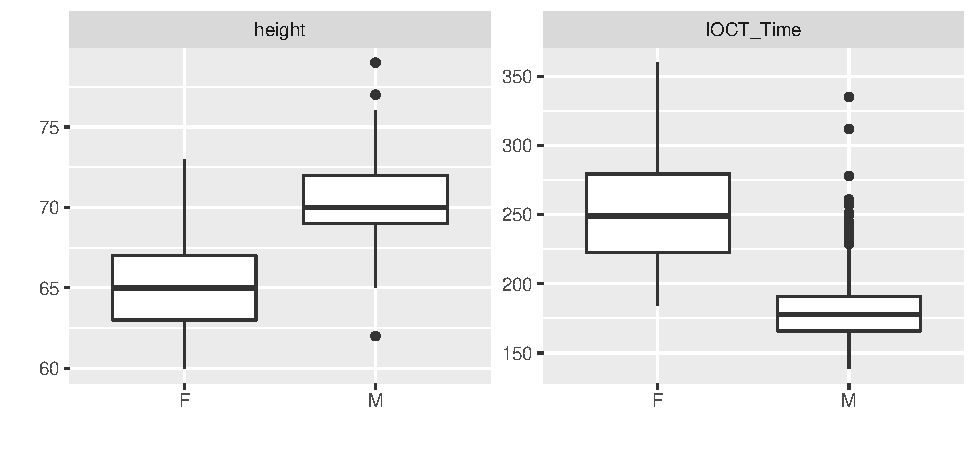
\includegraphics{MA206supplement_files/figure-latex/unnamed-chunk-3-1.pdf}
\caption{\label{fig:unnamed-chunk-3}Height (inches) and IOCT time (seconds) by sex.}
\end{figure}

\begin{enumerate}
\def\labelenumi{\arabic{enumi}.}
\setcounter{enumi}{12}
\tightlist
\item
  Based on Figure 2, is the estimate of the effect of height on IOCT time in Table 1 confounded by sex? If so, is the effect of height smaller or larger than that reported in Table 1? Explain.
\end{enumerate}

\vspace{1in}

\newpage

Figure 3 depicts the association between IOCT time and height by sex. Tables 2 and 3 depict regression results for female and male cadets, respectively.

\begin{figure}
\centering
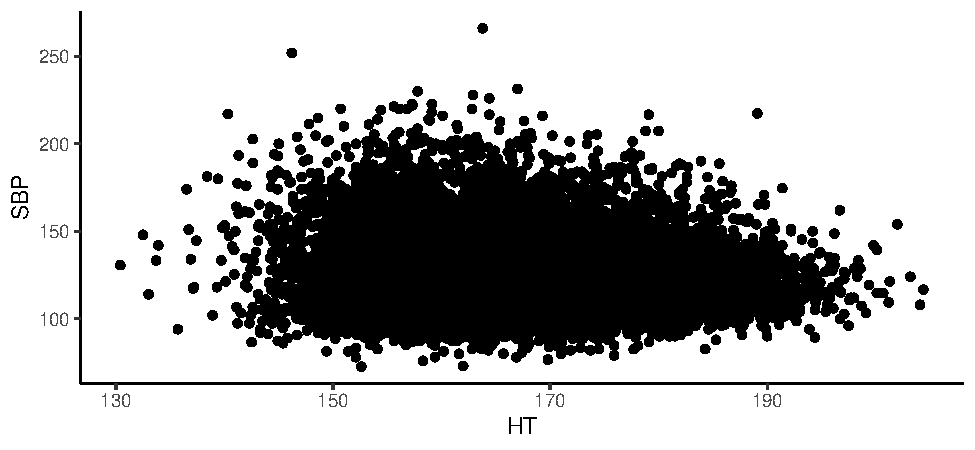
\includegraphics{MA206supplement_files/figure-latex/unnamed-chunk-4-1.pdf}
\caption{\label{fig:unnamed-chunk-4}Indoor Obstacle Course Test (IOCT) times versus height by sex (n = 384).}
\end{figure}

\begin{table}

\caption{\label{tab:unnamed-chunk-5}Regression results for female cadets.}
\centering
\begin{tabular}[t]{l|r|r|r|r}
\hline
term & estimate & std.error & statistic & p.value\\
\hline
(Intercept) & 335.76 & 107.44 & 3.12 & 0.00\\
\hline
height & -1.24 & 1.64 & -0.76 & 0.45\\
\hline
\end{tabular}
\end{table}

\begin{table}

\caption{\label{tab:unnamed-chunk-5}Regression results for male cadets.}
\centering
\begin{tabular}[t]{l|r|r|r|r}
\hline
term & estimate & std.error & statistic & p.value\\
\hline
(Intercept) & 175.61 & 40.92 & 4.29 & 0.00\\
\hline
height & 0.09 & 0.58 & 0.15 & 0.88\\
\hline
\end{tabular}
\end{table}

\begin{enumerate}
\def\labelenumi{\arabic{enumi}.}
\setcounter{enumi}{13}
\tightlist
\item
  Based on Figure 3 and Tables 2 and 3, does it appear there is an association between IOCT time and height within levels of sex? Explain.
\end{enumerate}

\vspace{1in}

\newpage

\begin{enumerate}
\def\labelenumi{\arabic{enumi}.}
\setcounter{enumi}{14}
\tightlist
\item
  In your opinion, is there much evidence that height is an advantage on the IOCT (in other words, is height the \emph{cause} of better IOCT times)? Explain.
\end{enumerate}

\vspace{2in}

\begin{enumerate}
\def\labelenumi{\arabic{enumi}.}
\setcounter{enumi}{15}
\tightlist
\item
  Briefly discuss two ways you could improve this study to better assess whether there is a height advantage.
\end{enumerate}

\vspace{1in}

\hypertarget{quantitative}{%
\chapter{(COL Watts) Quantitative explanatory variable with quantitative confounding variable}\label{quantitative}}

Explanatory (\(X\)) - quantitative

Response (\(Y\)) - quantitative

Confounding (\(C\)) - quantitative

\hypertarget{effect-of-x-and-y-adjusting-for-c.-1}{%
\section{\texorpdfstring{Effect of \(X\) and \(Y\) adjusting for \(C\).}{Effect of X and Y adjusting for C.}}\label{effect-of-x-and-y-adjusting-for-c.-1}}

\hypertarget{assessing-model-adequacy-1}{%
\section{Assessing model adequacy}\label{assessing-model-adequacy-1}}

\bibliography{book.bib,packages.bib}

\end{document}
